\subsection{Lights} % (fold)
\label{sub:lights}

This example draws three light bulbs to the screen. These lights can be clicked to turn them on and off. The code includes the declaration of a record/structure and an enumeration.

\begin{figure}[h]
   \centering
   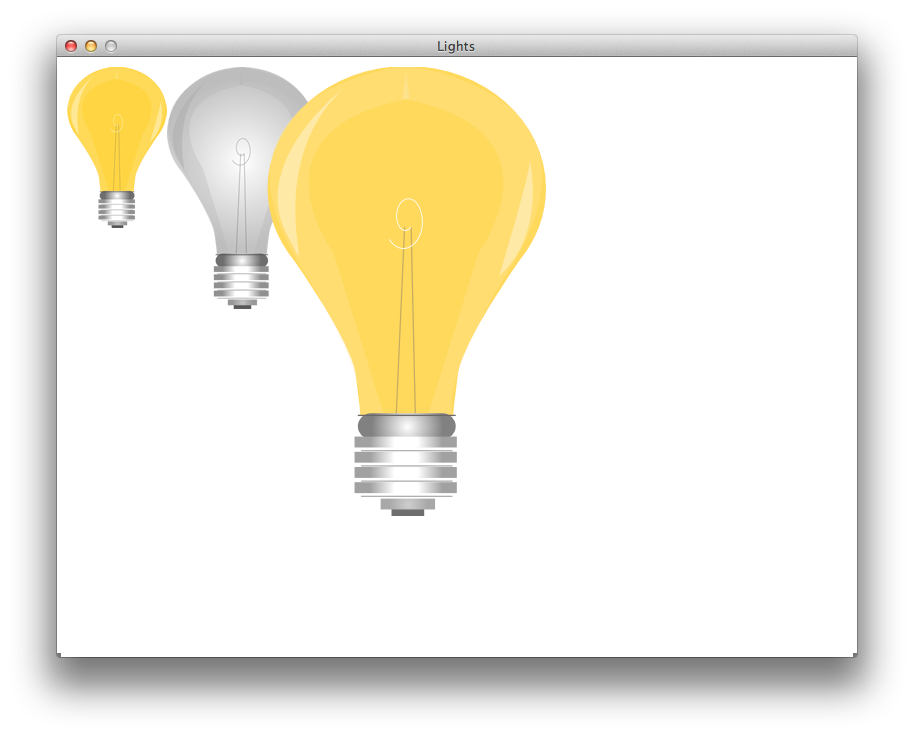
\includegraphics[width=0.8\textwidth]{./topics/type-decl/examples/Lights.png} 
   \caption{Example execution of the Lights program}
   \label{fig:lights-img}
\end{figure}

\clearpage

\cppsection{\ccode{cpplst:lights}{Lights code in C++, continues in \lref{cpplst:lights1} }{topics/type-decl/examples/lights.cpp}}

\cppsection{\ccode{cpplst:lights1}{Lights code in C++, continues in \lref{cpplst:lights2} }{topics/type-decl/examples/lights1.cpp}}

\cppsection{\ccode{cpplst:lights2}{Lights code in C++, continues in \lref{cpplst:lights3} }{topics/type-decl/examples/lights2.cpp}}

\cppsection{\ccode{cpplst:lights3}{Last of the Lights code in C++}{topics/type-decl/examples/lights3.cpp}}

\passection{\pascode{plst:lights}{Lights code in Pascal, continues in \lref{plst:lights1} }{topics/type-decl/examples/Lights.pas}}

\passection{\pascode{plst:lights1}{Lights code in Pascal, continues in \lref{plst:lights2} }{topics/type-decl/examples/Lights1.pas}}

\passection{\pascode{plst:lights2}{Lights code in Pascal, continues in \lref{plst:lights3} }{topics/type-decl/examples/Lights2.pas}}

\passection{\pascode{plst:lights3}{Lights code in Pascal }{topics/type-decl/examples/Lights3.pas}}

% subsection lights (end)
\clearpage
\subsection{Shape Drawing} % (fold)
\label{sub:shape_drawing}

The Shape Drawing program allows the user to create simple shape drawings using circles, triangles, rectangles, and ellipses. 

\begin{figure}[h]
   \centering
   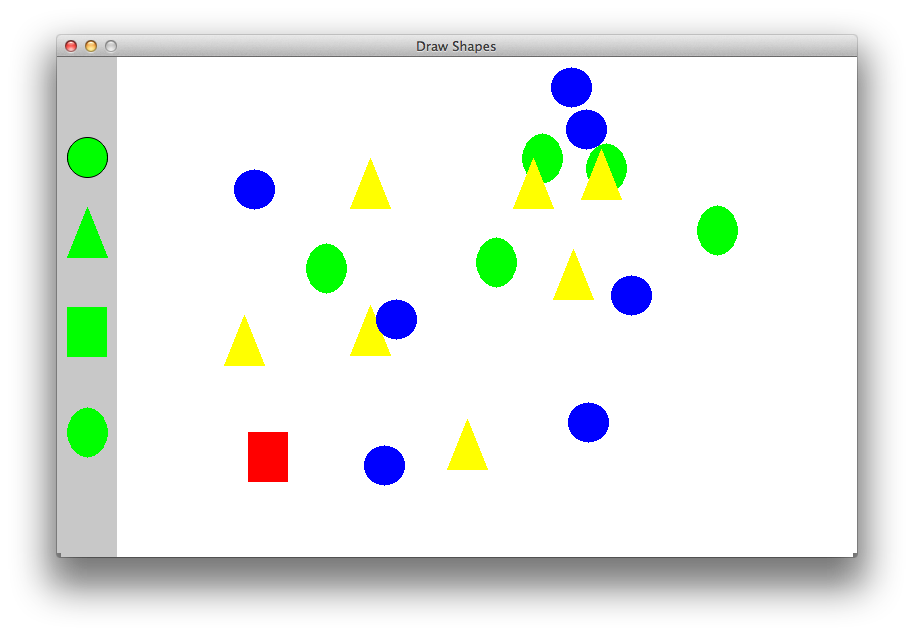
\includegraphics[width=\textwidth]{./topics/type-decl/examples/ShapeDrawing.png} 
   \caption{Example execution of the Shape Drawing program}
   \label{fig:shape-drawing-img}
\end{figure}

\clearpage

\cppsection{\ccode{cpplst:shape_drawing}{Shape Drawing code in C++, continues in \lref{cpplst:shape_drawing1} }{topics/type-decl/examples/shape_drawing.cpp}}

\cppsection{\ccode{cpplst:shape_drawing1}{Shape Drawing code in C++, continues in \lref{cpplst:shape_drawing2} }{topics/type-decl/examples/shape_drawing1.cpp}}

\cppsection{\ccode{cpplst:shape_drawing2}{Shape Drawing code in C++, continues in \lref{cpplst:shape_drawing3} }{topics/type-decl/examples/shape_drawing2.cpp}}

\cppsection{\ccode{cpplst:shape_drawing3}{Shape Drawing code in C++, continues in \lref{cpplst:shape_drawing4} }{topics/type-decl/examples/shape_drawing3.cpp}}

\cppsection{\ccode{cpplst:shape_drawing4}{Last of the Shape Drawing code in C++}{topics/type-decl/examples/shape_drawing4.cpp}}


\passection{\pascode{plst:shape_drawing}{Shape Drawing code in Pascal, continues in \lref{plst:shape_drawing1} }{topics/type-decl/examples/ShapeDrawing.pas}}

\passection{\pascode{plst:shape_drawing1}{Shape Drawing code in Pascal, continues in \lref{plst:shape_drawing2} }{topics/type-decl/examples/ShapeDrawing1.pas}}

\passection{\pascode{plst:shape_drawing2}{Shape Drawing code in Pascal, continues in \lref{plst:shape_drawing3} }{topics/type-decl/examples/ShapeDrawing2.pas}}

\passection{\pascode{plst:shape_drawing3}{Last Shape Drawing code in Pascal }{topics/type-decl/examples/ShapeDrawing2.pas}}


% subsection shape_drawing (end)